\documentclass[12pt]{article}

\usepackage{epsfig}
\usepackage{comment}
\usepackage{natbib}
\usepackage{natbibmnfix}
\usepackage{graphicx}
\usepackage{color}
\usepackage{subfig}
\usepackage{bmpsize}
\usepackage{caption}
\usepackage{amsmath}
\usepackage{breqn}

\newcounter{dummy}
\def\@biblabel#1{\hspace*{\labelsep}[#1]}

\newcommand{\df}{\delta_{\rm F}}


\def\lya{Ly$\alpha$}
\def\lyb{Ly$\beta$}
\def\etal{{\rm et~al.\ }}
\def\hmpc{\;h^{-1}{\rm Mpc}}
\def\hgpc{\;h^{-1}{\rm Gpc}}
\def\hkpc{h^{-1}{\rm kpc}}
\def\kpc{{\rm kpc}}
\def\kms{{\rm \;km\;s^{-1}}}
\def\shear{\langle \gamma^{2} (\theta) \rangle}
\newcommand{\phiv}{\mbox{\boldmath$\phi$}}
\newcommand{\thetav}{\mbox{\boldmath$\theta$}}
\def\pef{\par\noindent\hangindent 15pt}
\def\simlt{\lower.5ex\hbox{$\; \buildrel < \over \sim \;$}}
\def\lesssim{\lower.5ex\hbox{$\; \buildrel < \over \sim \;$}}
\def\simgt{\lower.5ex\hbox{$\; \buildrel > \over \sim \;$}}
\def\apj{{\it Astrophys. J.}}
\def\aj{{\it Astron. J.}}
\def\mnras{{\it Mon. Not. R. astr. Soc.}}
\newcommand{\apjl}{ApJL}
\newcommand{\nat}{Nature}
\newcommand{\araa}{ARA\&A}
\newcommand{\apjs}{ApJS}
\newcommand{\aap}{A\&A}
\newcommand{\pasp}{PASP}
\newcommand{\sfig}[2]{
\begin{center}
\includegraphics[width=#2]{#1}
\end{center}
        }
\newcommand{\Sfig}[2]{
    \begin{figure}[htb]
    \sfig{./#1.jpg}{.5\columnwidth}
    \caption{{\small #2}}
    \label{fig:#1}
    \end{figure}
}
\newcommand{\Sfigtwo}[3]{
        \begin{figure}[htbp]
\sfig{#1.eps}{.3\columnwidth}
\sfig{#2.eps}{.3\columnwidth}
\caption{{\small #3}}
\label{fig:#1}
\end{figure}
}
\newcommand\be{\begin{equation}}
\newcommand{\Rf}[1]{\ref{fig:#1}}
\newcommand{\rf}[1]{\ref{fig:#1}}
\def\ee{\end{equation}}
\def\bea{\begin{eqnarray}}
\def\eea{\end{eqnarray}}
\newcommand{\vs}{\nonumber\\}
\newcommand{\ec}[1]{Eq.~(\ref{eq:#1})}
\newcommand{\Ec}[1]{(\ref{eq:#1})}
\newcommand{\eql}[1]{\label{eq:#1}}
\newcommand\cov{{\rm Cov}}
\newcommand\cl{{\mathcal{C}_l}}
\usepackage[margin=3.0cm]{geometry}
\usepackage{pslatex}
\newcommand\fnl{f_{\rm NL}}
\newcommand{\wh}[1]{\textcolor{blue}{[#1]}}

\newcommand\cp{C^{pri}}
\newcommand\ci{C^{ISW}}
\newcommand\cg{C^{gg}}
\newcommand\cgt{C^{g-ISW}}
\newcommand\tob{T^{\rm obs}}
\newcommand\aob{a^{\rm obs}}
\newcommand\tisw{T^{\rm ISW}}
\newcommand\aisw{a^{\rm ISW}}
\newcommand\si{C^{\rm ISW}_l}
\newcommand\sig[1]{C^{\rm g_{#1}-ISW}_l}
\newcommand\sg[2]{C^{\rm g_{#1}g_{#2}}_l}
\newcommand\tp{T^p}


%
% definitions
%
% A useful Journal macro
\def\Journal#1#2#3#4{{#1} {\bf #2}, #3 (#4)}
% Some useful journal names
\def\NCA{\em Nuovo Cimento\ }
\def\NPB{{\em Nucl. Phys.} B\ }
\def\PLB{{\em Phys. Lett.}  B\ }
\def\PRL{{\em Phys. Rev. Lett.\ }}
\def\PRD{{\em Phys. Rev.} D\ }
\def\prd{{\em Phys. Rev.} D\ }
\def\ZPC{{\em Z. Phys.} C\ }
\def\apj{{\em Ap. J.\ }}
\def\apjl{{\em Ap. J. Lett.\ }}
\def\la{\hbox{${_{\displaystyle<}\atop^{\displaystyle\sim}}$}}
\def\ga{\hbox{${_{\displaystyle>}\atop^{\displaystyle\sim}}$}}



\baselineskip=11pt
\def\msun{{\rm M_{\odot}}}

\textheight=24.3cm
\textwidth=16.8cm

\begin{document}
\topmargin=-2.105cm
\oddsidemargin=-0.1cm
\evensidemargin=0cm

\begin{center}
{\LARGE \bf New weak lensing tracers for precision cosmology}
\end{center}

\begin{small}



\section{Overview and Objectives}
Weak gravitational lensing has emerged as one of the powerful probes
of cosmology. The small distortions of background images as
they are lensed by foreground matter are sensitive to both the
contents and the geometry of the Universe (e.g., \cite{blandford92},
\cite{hoekstra2008}).  Galaxy images are the most commonly used
cosmological sources (see \cite{Kilbinger2015} and references
therein), but weak lensing of the cosmic microwave background (CMB) is
also widely studied (see e.g., the review by \cite{lewis2006}, and
results from, e.g., the Planck satellite, Ade {\it et al.} 2015).
 These two implementations of lensing differ not only 
in the sources 
studied  but also in
the fundamental observable. In one case,
 the shapes of galaxies are used to
determine the intervening gravitational potential (see the top
left panel in Figure 1, which shows galaxy clusters and large-scale structure).
On the other hand, for the
CMB, the potential can be mapped (middle panel of Figure 1) using
{\it anisotropies} in the
two-point statistics of the otherwise Gaussian field. 


These {\it anisotropic two-point functions} (hereafter \atf) will 
affect any cosmologically distributed background
sources. The field of weak lensing can therefore be broadened by looking 
at new applications of them. We choose three to work  on in this proposal:

{\bf(1) The \lya\ forest}- as the angular 
positions of quasars are deflected, the forest 
in quasar spectra is also lensed.
In \cite{croft17} (hereafter C18)
 the PI proposed measurement of the 
\atf\ of the \lya\ forest.


 {\bf (2) The \atf\ 
of the angular galaxy distribution}
relies on the same physics. The positions
of galaxies are deflected by lensing
resulting in local distortions of
clustering statistics.

{\bf (3) A new window on time delays with \atf}.So far, time delays have been
detected only in the case of strong lensing. But using our new
technique,  upcoming CMB experiments can estimate the time
delay field.



\Sfig{table}{\footnotesize{New vistas: anisotropies of the 2-pt. function 
in  galaxy clustering, CMB time delay, and the \lya\ forest}
}
\vspace{-0.1cm}


We will carry out an in depth study of these three new weak lensing
 applications of \atf\, spanning theory and 
simulations, from first detections to precision cosmology. We will study 
them together
 in order to benefit from
their common aspects, and common
simulations. Our specific objectives are as follows:

(a) {\bf \underline{to simulate new lensing tracers,}} the forest, galaxy clustering and time delay anisotropy,
 including non-linear physics, baryonic effects and observational
systematic errors.

(b) {\bf \underline{to develop statistical techniques}} for the analysis of new lensing data, including 
cross-correlations and mass reconstruction, and use knowledge from our full simulations to address and mitigate systematics.

(c) {\bf \underline{to make observational measurements}} from first 
detections to competitive  determinations of $\sigma_{8}$ at the 3\% level 
from forest and galaxy datasets, the CLAMATO, eBOSS and DES surveys.

(d) {\bf \underline{to explore new cosmological constraints}} from these
measurements which have different strengths and potential biases  to other
lensing results.



including star formation and black holes.

\subsubsection{Combined models}
By mapping sections of hydrodynamic simulations onto a much larger
dark matter simulation (or even linear density fields) it is possible
to accurately reproduce many of the features of the \lya\ forest
in a larger hydrodynamic simulation. This
technique was used successfully by \cite{croft2004} and developed in
detail by \cite{peirani2014}. We have all the relevant 
simulation ingredients and will adopt this approch.

\subsection{\lya\ forest source Mocks}
\lya\ forest spectra will be made by integrating through the
neutral hydrogen distribution ( in SPH kernels in the case of the hydro
simulations)
along each sightline and then convolving with the line-of-sight velocities
and applying thermal broadening \citep{hernquist1996}.
 In order to make realistic
mock catalogs we will use the relevant observational parameters
of different datasets from Table\ref{obs}. Quasar and galaxy sightlines will
be picked randomly with the correct mean spacing. In our test so far
(C18) we have used a grid of background sources, which is obviously
unrealistic, and so an important part in our proposed work is to abandon
that simplification. Apart from survey geometry we will investigate
the role of uncertainties in  quasar and galaxy continuua. We will 
apply continua based on published principal components
of quasar spectra \citep{leedr9} and population synthesis models
to the mocks, before fitting them using low order polynomials. This will
enable us to estimate the covariance between pixels on large-scales which
are due to continuum fitting.


\subsection{Galaxy sources}
\label{galaxysourcesims}
In our study of LIA it is important to resolve large-scale structure
in the galaxy distribution but galaxy shapes themselves are not needed.
A number of suitable N-body simulations are therefore 
available to use, for example
those used in \cite{zhu2017} (see Table \ref{tab_runs}, and we will use a HOD 
approach (e.g,) to populate the dark matter distribution with galaxies.
Although angular clustering will be measured, we will make use of the 
three dimensional information in the simulations to assign photometric
redshifts and model systematic uncertainties related to their use in 
the presence of errors, catastrophic and otherwise \citep{hearin2010}.
Hydrodynamic simulations of small volumes are also available 
(Table \ref{tab_runs}) and
will be used as the source fields in lensing simulations of individual
galaxy clusters in order to investigate baryon physics effects.


\subsection{Simulated lenses}
In situations such as forest lensing with widely spaced sightlines,
the 
the lensing field will be detected only on large angular scales 
where the matter structure responsible for the lensing is linear to a
reasonably good approximation. Our lens simulations (e.g. C18)
have started from the simplest case, a Gaussian random field.   
We create a realization of the lensing potential by generating random 
Gaussian  distributed Fourier modes with the power spectrum expected 
in the same cosmology
 used to simulated source fields.   The deflection is found by taking the 
gradient of the potential using an FFT.  Points on the source planes 
are then displaced by the deflection to get the lensed image. 
In the case of the forest, the deflection is applied to individual pixels
(see Figure 1) in the forest source simulations
 and for LIA to galaxies described in Section \ref{galaxysourcesims}
We will start with a single lens plane approximation for the forest lensing
case based on the linear fields. For the LIA with a cluster lens, the 
simplest initial simulations will be of a single spherically  symmetric lens.

In order to capture the true non-linearity inherent in the lens field,
 we will then move to using ray-traced  Nbody simulations. We have chosen  
GLAMER   \cite{metcalf2014} to do this (collaborator Ben Metcalf is an 
author of the code). It incorporates adaptive mesh refinement for
efficient choice of ray shooting. The deflection and beam distortions 
(convergence and shear) are calculated by modified tree algorithm when haloes,
 point masses or particles are used and by fast Fourier transform when 
mass maps are used. The combination of these methods allow for a very 
large dynamical range, so that accurate  maps will be made
spanning several degrees and covering large-scale
structure in the lensing matter distribution. Multiple lens planes can be
handled by GLAMER \cite{petkova2014}, and the distribution of matter
will be taken from the simulations detailed in Table \ref{tab_runs}. A suite 
of publicly available raytraced simulations (the Multi Dark Lens Simulations,
\cite{giocoli2016}) has been carried out and will also be used for 
this project. These include over 150 realizations of $\sim 10$ square
degree fields carried out using fully sampled lightcone raytracing
with 24 lens planes each. The simulations therefore cover both the
redshift $z\sim1$ lenses relevant for forest lensing and the lower 
redshift needed for LIA in the same simulation. They can be used to
test both, and in principle look at the overlap in lensing reconstruction
(and lensing kernels) for the two methods. 


\subsection{Full mocks}

Given the simulated sources and lens described above, we will construct
full mock datasets where we mimic the geometry and noise properties
of particular datasets. These datasets are detailed below in Section 6.
We note that because some of them are extremely large in
angular extent (e.g. eBOSS and DES), we will make use of a combination of
small high fidelity mocks of sections (for example individual 
galaxy clusters) and others larger areas generated using the approximate 
techniques mentioned above.
We will also incorporate addition levels of
complexity and potential sources of systematic
error, treating the addition of each in turn. For both types of
lensing we consider, magnification will be important, as both source
galaxies and background quasars will be selected preferentially when
they are lensed. The effects of photometric redshift uncertainties
could also  be added 
at this stage.   


\section{Planned work: Estimators}

Reconstructing the lensing mass distribution from observations
(and making maps, or measuring
clustering statistics or object properties directly) requires  an
estimator. 
A quadratic lensing estimator (e.g., \cite{okamoto}) for the forest or for LIA
is sensitive to variations in the power spectrum in  different 
regions of the sky.  These spatial variations result in
correlations in Fourier modes (or $C_\ell$'s) that would not
exist otherwise. 
In our proposed work, we will further develop estimators
of the type that have been applied to the CMB but specialized to our
new tracers (for example the discrete sightlines of the \lya\ forest).

\subsection{Estimators for Lensing anisotropy of galaxy clustering}

In the case of LIA we will be concentrating first on detecting and
measuring the lensing signal of stacked galaxy clusters..
The simplest estimator to try first is a parametric model with,
e.g., the mass and concentration of the clusters set as free
parameters. The data points will be   $N_{\rm pix}^2/2$
estimates of $\hat w$, and these
can be used to constrain the parameters.
We will also explore maximum likelihood methods
that do not rely on the small angle approximation.

\subsection{Estimators for \lya\ forest lensing}
In C18 it was found that the standard quadratic estimator works 
very well on gridded spectral \lya\ forest data. As real
galaxies and quasars do not exist on a grid, the challenge is
to develop an estimator that works on a random discrete set of sightlines.
Several different approaches can be taken, the simplest being an interpolation
of the data onto a finely space uniform grid. We have experimented with this
approach, finding that it could be useful in conjunction with the detailed
simulation tests proposed above to establish how interpolation errors 
propagate. However, the PI, together with collaborator Ben Metcalf has 
developed a quadratic estimator which uses non-gridded data 
(\cite{metcalf17}). Without a grid, FFT methods are not available to 
speed up the estimator, but inversion of large matrices is required. At 
present tests on small (million pixel) simulations have shown success and
during this proposal we will improve the code and scale up to the capabilities
needed to process full mock and observational datasets.

\subsection{Mitigating systematics: the road to precision cosmology}

Our simulation tests with realistic sources and lens fields will reveal the extent to which non linearity and non Gaussianity
affect the lens reconstructions. We will seek to develop methods to mitigate these effects. For example, in CMB lensing \cite{lewis16} have shown how the effects of non Gaussian deflections from post-Born corrections and non-linear structure growth can be can be severely reduced by Gaussian smoothing. Also for CMB lensing, \cite{bohm18} have shown that results from raytraced simulations can be accounted for and corrected using  analytic results (\cite{bohm16}). Although in the CMB these issues are at the $\sim0.3 \%$ level in the power spectrum, they will be a more significant issue with our lower redshift lensing tracers and should be addressed as we seek to develop them as new tools for precision cosmology. We will use the CMB lensing work as a guide to push the precision of our work to below the level of the simulated systematics.

\subsection{Cross-correlation and validation}
As our lensing techniques are new, an important part of our studies will
be checking results against relevant prior data.
Measurement of cross-correlations with foreground galaxies or CMB
lensing maps are likely to consistute the first proof that our
techniques are valid.
 In the case of forest lensing,
foreground galaxy maps are available for large areas of the sky from the
SDSS/BOSS and eBOSS surveys. We can use the distribution of galaxies 
(LRGs and ELGs from eBOSS) with redshifts,
weighted by the lensing kernel to make a predicted lensing
convergence  map. We will
 cross-correlate this map with convergence estimated from the forest. 
We will test this cross-correlation with our mock catalogs, and use
them to quantify systematic errors. In the case of LIA galaxy
clusters selected from photometry itself play the largest role,
and again the mocks will be important to bracket uncertainties 
(such as the role of baryonic physics  \cite{zentner2013}).



\section{Planned work: Observational measurements}

The new weak lensing tracers we are proposing are unusual in that
observational data already exists which could allow high
significance detections and precise constraints on cosmology. We
therefore plan to move rapidly  to make first detections alongside
our work on mock catalogs,  using those mocks to
inform our estimates of errors and uncertainties.



\begin{figure}
 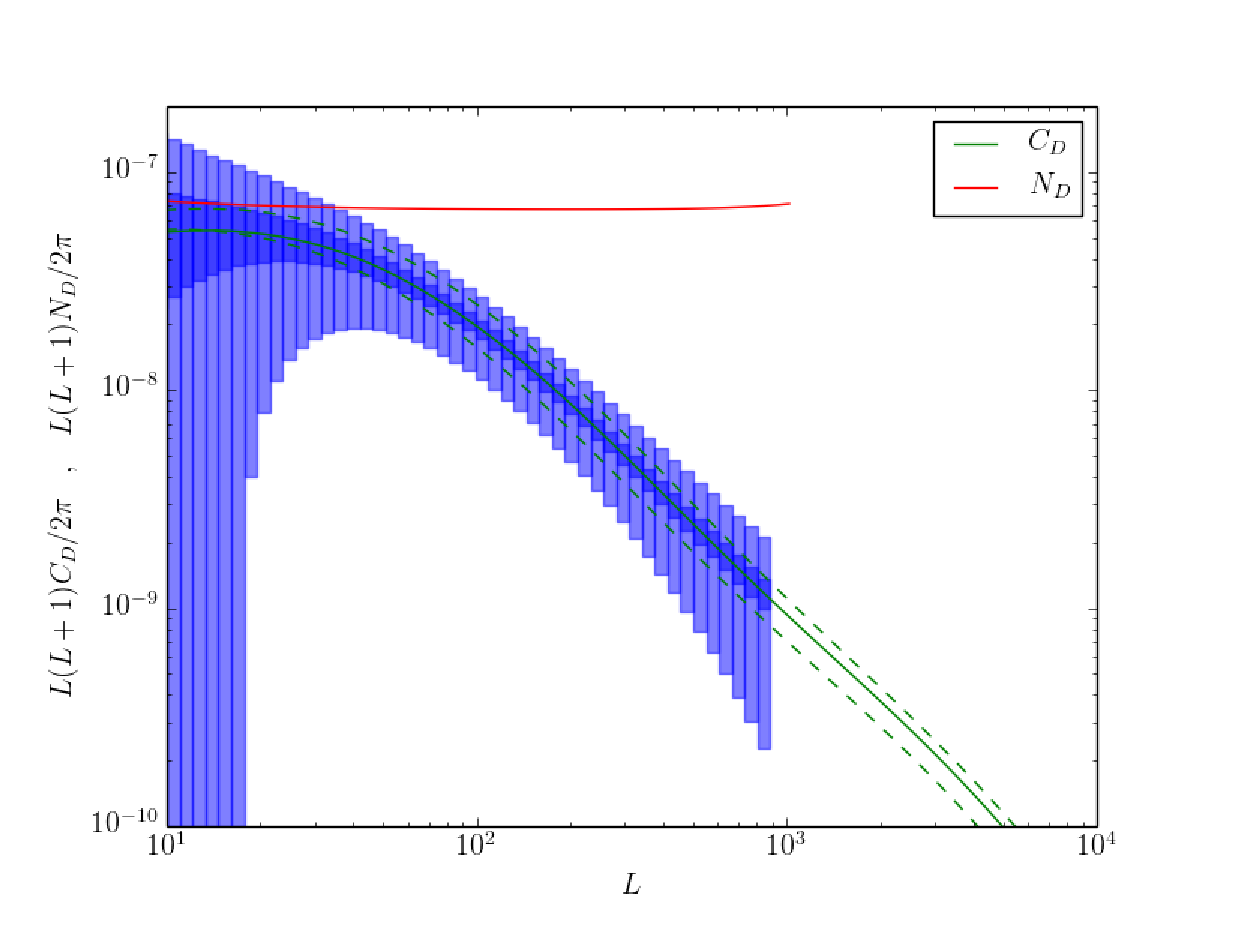
\includegraphics[width=0.5\columnwidth]{eBOSS.eps}
 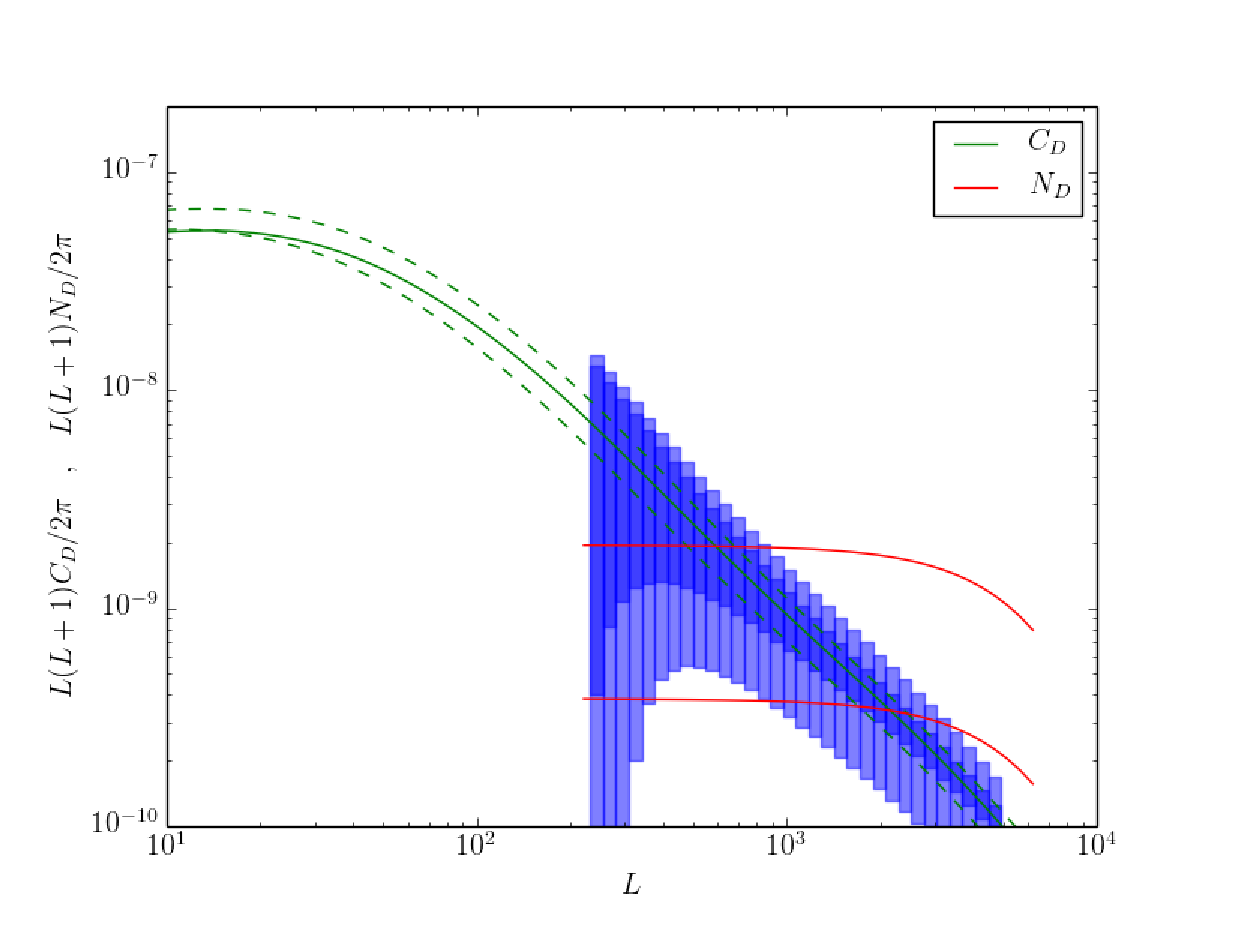
\includegraphics[width=0.5\columnwidth]{CLAMATO.eps}
 \caption{ {\bf The predicted lensing displacement power spectrum  measured
from the \lya\ forest and its 
estimated errors. }
{\bf Left panel:}
eBOSS survey  (see Table~\ref{obs}). The smaller errors are for a redshif
t range $\Delta z =0.5$ and the larger for $\Delta z = 0.1$.  For this survey,  $N_D$ (the noise per 
mode, red line)  is off the range of the plot.  The green curves labelled $C_D$ show the expected power spectra, with the solid curve being for $z_s=2.5$.  For comparison, the upper dashed green curve s
hows results for $z_s=3$ and the lower one for $z_s=2$. {\bf Right panel:}
The CLAMATO survey (\ref{obs}).
The two red curves are the noise in each mode, $N_D$, for the $\Delta z =0.5$ (lower) an
d $\Delta z = 0.1$ (higher) cases.  Where $N_D$ is below $C_D$ high fidelity maps of the lensing convergence is possible.}

 \label{pkpred}
\end{figure}



\begin{table}
\begin{tabular}{|l|l|l|l|l|}
\hline
Dataset   & When      & Area            & N_{\rm spectra} & mean separation \\ \hline
BOSS DR12 & 2016      & 10,000 sq. deg. & 160,000            & 15 arcmin       \\
eBOSS     & 2014-2020 & 7,500 sq. deg.  & 270,000            & 10 arcmin       \\
CLAMATO   & 2014-2020 & 0.8 sq. deg.    & 1,000              & 1.7 arcmin      \\
\hline
\end{tabular}
\centering
\caption{
{\bf \lya\ forest observational
datasets we will use.} 
Of these, BOSS (Dawson {\it et al.} 2013) has been completed,
eBOSS (Dawson {\it et al.} 2016) and CLAMATO (Lee {\it et al.} 2014, using
galaxy spectra) are ongoing. }
\label{obs}
\end{table}



\subsection{The CLAMATO survey: first detection of \lya\ forest lensing}

The COSMOS Lyman-Alpha Mapping And Tomography Observations (CLAMATO,
\cite{clamato})
 survey is a dense sampling of \lya\ forest spectra in the
COSMOS field, using both quasars and galaxies as backlights.
Some characteristics of the survey are given in Table\ref{obs}. The
sightline density is such that one can expect to make high
fidelity maps of the foreground lensing mass once the survey is completed.
An approximate idea can be gained from Figure \ref{recon} where we show
tests of the reconstruction technique from C18 where the sightline
density was similar to that in the CLAMATO survey. 
CLAMATO has had its first public data release \cite{clamato} and
we will use this data to make what is likely to be the first 
detection of \lya\ forest lensing. A prediction of the 
signal to noise expected in a determination of the lensing mass power spectrum
(taken from the PI's work 
\cite{metcalfandcroft}) is shown in Figure\ref{pkpred}. For
the full survey we expect an 6 \%  constraint on the amplitude
of mass fluctuation $\sigma_{8}$. The first data release contains about
one third of the hoped for final dataset. Galaxy densities are available
to high redshift in the COSMOS field meaning that validation of the
measurement with cross-correlation should be straightforward.

\begin{figure}
  \begin{center}
    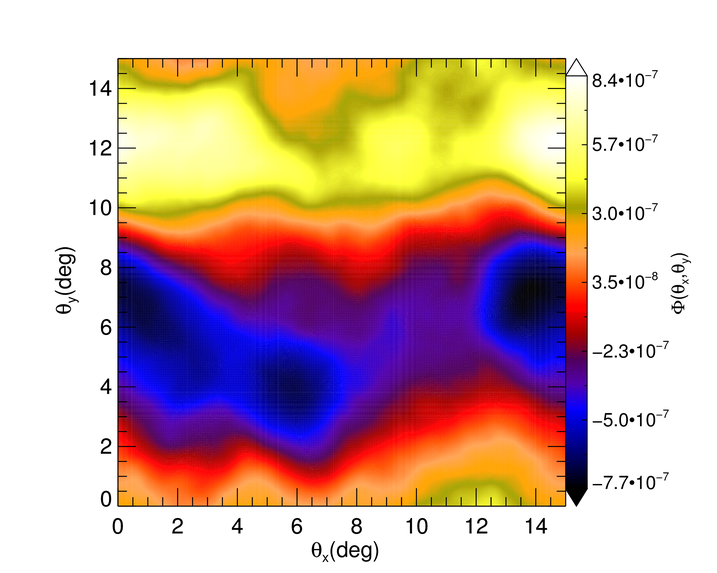
\includegraphics[scale=0.3]{GRP_512_15_z1.png}
    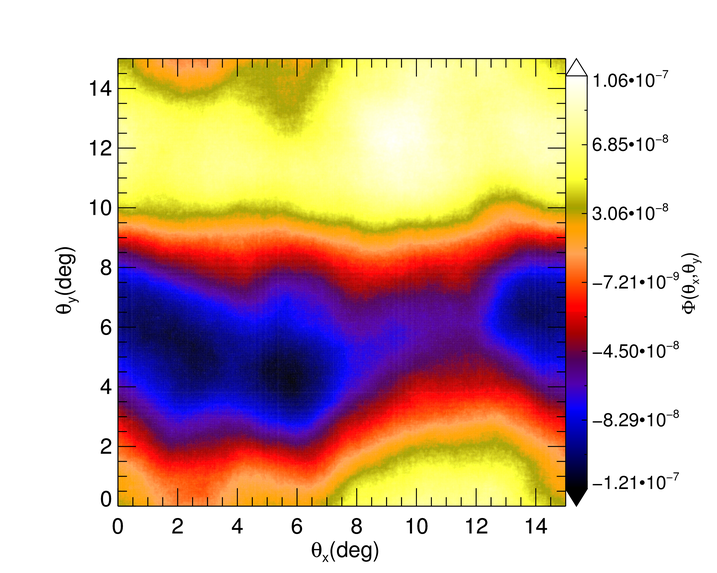
\includegraphics[scale=0.3]{GRP_512_15_z1_Recov.png}
  \end{center}
  \caption{
{\bf Recovery of the lensing potential field from a simulation of \lya\ forest
lensing}. The left panel shows the input potential and the right panel
the potential reconstructed from a lensed \lya\ forest dataset. The plot is taken from C18, and used gridded forest data (something which will
be improved in our proposed work). The mean spacing of sightlines was 
comparable to that in the CLAMATO survey, which we plan to analyze.
           }
  \label{recon}
\end{figure}

\subsection{eBOSS: 3 percent precision on $\sigma_{8}$}
The eBOSS survey is ongoing, but has completed more than two thirds its survey
footprint and will be complete early in our project.
It is a large area, low sightline density survey (see Table\ref{obs}), so
that foreground mass maps will have low fidelity. The large area will
however lead to a precise measurement of the power spectrum.
The right panel of Figure \ref{pkpred} shows our prediction from 
\cite{metcalfandcroft}, which yields a 3\% measurement of $\sigma_{8}$.

\subsection{DES clusters: first detection of lensing anisotropies in
galaxy clustering}

Once tested on simulations, we will apply our
LIA method to clusters in the Dark Energy Survey \cite{des2016},
for which the Co-I is co-Chair of the Science Committee. 
As we have shown in Section \ref{sec:lia}, ample signal to noise will be
available given the more than tens of  thousands of galaxy clusters 
that will be selected using the redMaPPer algorithm~\cite{melchior2017}.
Comparison will be made to the shear-based
mass measurements of the same clusters \cite{simet2017} and with
estimates of their mass inferred from the angular clustering
of clusters \cite{baxter2016}.
The estimator codebase developed and used on DES data will
be released to the community so that it can be used, for example, by
all members of the LSST Dark Energy Science Collaboration.

\section{Planned work: Cosmology}

A significant part of our effort will be devoted to identifying ways 
in which our new lensing tracers can be advantageous to cosmology.
As an example, we will compute neutrino mass constraints using the
measurements. We will investigate how the new cluster mass determinations
(and the checks they provide on systematic errors in other methods)
propagate into estimates of dark energy parameters. In general, new probes
of the dark matter distribution which have no dependence on galaxy shape 
measurements, will have many advantages. The \lya\ forest with its automatic
full redshift information could also be used
to carry out tomography of the foreground matter, or measure the amplitude
of clustering at different redshifts (see the green lines in Figure 
\ref{pkpred}), and this can also be used to constrain dark energy. We note 
that  we  have not considered self-lensing by the forest (\cite{loverde2010}),
and this may offer a path to other, differing constraints.


\section{Broader impact and outreach}

The best outreach program should be able to easily reach women and
minority groups underrepresented in science. Video games provide
a good way to do just that- a  study from the  Pew Internet 
\& American Life 
Project (Lenhart 2008) found that the percentage of American youth
that play video games is almost the same for a wide range of racial and
ethnic groups and incomes. The survey combined the telephone responses 
from a nationally representative sample of 1,102 young people, ages 12 to 
17, and their parents. It found that 99\% of boys and 94\% of girls
play video games, and they play them often, with  half of the respondents 
saying they had played a video game the previous day. This adds up to
over 200 million person-hours of video gaming each day in the U.S.

Games are clearly entertaining as judged by their use, 
but what if they had educational benefits? 
Our proposal 
focuses not on general computer and video games, but on educational games,
and the ideas we incorporate are 
grounded in a theory of intrinsically motivating instruction 
based on a rigorous study of educational games 
(Malone 1981, Gee 2003,
Squire 2003, Aldrich 2004, Schell 2008).


Through the medium of  games, our outreach aims are the following:\\
\noindent {\bf (1a)} To introduce  elementary and middle
school students to the length scales relevant
to astronomy, from the Solar system to the large scale structure of the Universe
.\\
\noindent{\bf (1b)}  To introduce school children to the chemical constituents
 of the Universe and how they are distributed on Astronomical scales.\\
\noindent{\bf (1c)} To introduce high school students to the concept
of quasars, the  intergalactic medium and absorption lines.\\
{\bf (2)} To provide an interactive 
learning experience. The best way to learn is
to make it an enjoyable  experience from the start. We do not
however want people to take part necessarily
because they want to learn about these
topics. Being entertained is enough, and familiarity with these topics
will come about through the way the game is designed.\\
{\bf (3)}
To reach the largest audience possible. Given that only small fraction of 
the target audience is familiar with  the above concepts  we take the view 
that 
there is a huge amount to be gained from disseminating even simplified 
knowedge among a number of people which is enormous compared to the usual 
outreach channels (lectures  etc..). The gains of this broader 
impact would be to increase interest in science as a career across 
a desirable demographic.
  

\subsection{Minecraft Astronomy lesson plans}




We propose to make lesson plans for elementary and middle school students to 
learn the size scales of the Universe and understand the elemental content 
of the Universe using the popular game Minecraft. 
Minecraft is akin to digital Lego bricks – players inhabit a 
three-dimensional 
world of blocks with its own unique ecosystem and physical laws. Using 
imagination, 
players build whatever they can dream up by mining resources, combining, 
and placing them to build everything from pickaxes 
to complex and working electrical systems. So far, 100 million people have 
purchased 
the Mac/PC version of the game. 
It is considered a sandbox game, providing nearly limitless opportunities 
to  build. Teachers can buy discounted licenses through MinecraftEdu.com, as 
well as a plug-in to tailor the software to a specific curriculum. 



\begin{figure}%[ht!]
\centering
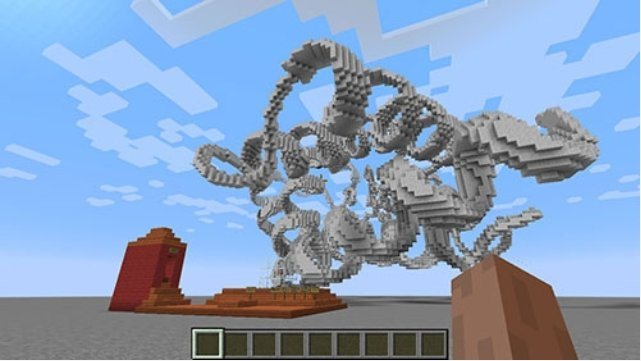
\includegraphics[width=75mm]{myoglobin.jpg}
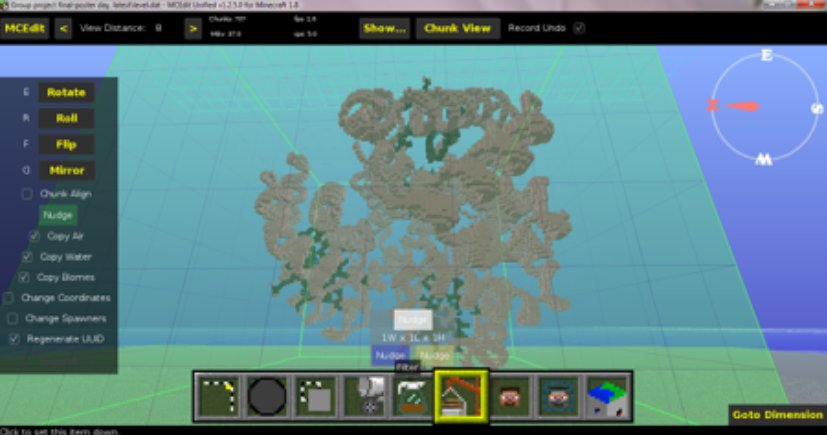
\includegraphics[width=80mm]{mcedit.jpg}
\caption{\footnotesize{{\bf Left:
Minecraft visualization of myoglobin molecule} 
Reproduced from the MolCraft project, University of Hull, UK
{\bf Right: Importing three dimensional structure into Minecraft
using MCedit} Reproduced from the MolCraft project, University of Hull, UK
}}
\label{molcraft}
\end{figure}


As an educational tool, Minecraft teaches design, collaboration, co-creating 
and problem solving. It’s an active learning environment. Previously, 
successful
 physics lessons have been created for studying quantum mechanics 
(q-Craft Curriculum Project) and testing gravity (Rhett Alain, Wired) in 
Minecraft. Gamers enjoy making maps, building things and solving puzzles. 
Our 
Minecraft Astronomy elementary school tutorial will give instructions on 
how to 
build a rocket and how to use it to navigate a map of the Universe hosted 
on our server. Our middle school tutorial will include plans to build a 
telescope and 
how to use it to find the atoms that make up our Universe. Self-driven 
inquiry 
leads to locations on our maps where the content is kept up-to-date.
 Blog 
posts will connect users, guide them in reflective, 
“big picture” 
thought processes, craft intuitive thinking and inspire their natural 
curiosity. 
Astronomy facts, paired with math, cosmic pictures and stories will 
enrich learning.
 
One lesson plan will be primarily for 1st to 4th graders and will focus on the s
ize scale of the solar system.
We have substantial experience in this topic as the PI has been
carrying outreach to this demographic since 2002, as part of the CMU
Physics department's outreach program. Some of the outreach activities
involved making scale models of the solar system with household objects. 
Several limitations can be overcome by using the Minecraft world to do this, 
including  extending the scale of the models arbitrarily, and using the 
3rd dimension.
 A second lesson plan will focus on the atomic content of 
the Universe for middle school students (5th to 7th grade). Game users 
will hunt to  find the rare metals among the hydrogen and helium 
atoms of the universe, finding 
the prized heavy elements in places like rocky bodies and supernovae remnants. 
We will develop worlds based on several different length scales, including
one where we will import galaxy redshift survey data (from the SDSS) so that 
the students can fly around and explore 
the large scale structure of the Universe.
It is simple to import such data sets and edit them- an example
of biological molecules taken 
from the Molcraft project (University of Hull, UK) is shown in Figure 
\ref{molcraft} and it is easy to imagine how astronomical data would work
in this environment.


Overworld dimensions of the square game plane are $3.59 \times 10^{9}$
 square kilometers 
(as compared to the Earth’s spherical $5.09 \times 10^{8}$
 square kilometer area). 
The height  is 256 blocks, but a Sky Dimension of similar size to the 
Overworld is 
planned for a future release. A shared world will be created and gamer guides 
released to aid exploration. For teachers, lesson plans will be made, 
including 
objectives and goals based on educational standards, a prior knowledge test, 
directed instruction, vocabulary definitions, guided practice sets and an assess
ment 
worksheet. As our work progresses, we plan to bring these lessons to a local 
school 
for tests with students.
These include such schools as Colfax School, Milliones School and Helen Faison
academy which we have worked with before, and where there are high fractions
of students from minorities underrepresented in science.
 While these lessons will be available to the 
general public, they will be geared toward educators to be used in classrooms.

\subsection{Universe Sandbox Tutorial}


For high school students, 
we propose using the commercial software Universe Sandbox2 
 (universesandbox.com) to build a Lyman-alpha forest tutorial 
and activity. 
Universe Sandbox is an interactive space simulator, giving players the ability t
o 
wander through sections of the known universe. Universal Sandbox2 is a fully 
featured, space simulator, with new features and simulations added 
based on community requests. Players have the ability to observe and 
change the universe by altering fundamental constants (like the strength of 
gravity) and by moving celestial objects through space and time. 
Our high school and introductory college astronomy lesson will walk 
students through a Lyman-alpha forest simulation to show intervening 
material at differing redshifts. The material creates a forest of absorption 
lines and the tutorial will explain how that is seen in the visual in quasar 
spectra, using diagrams and an interactive applet that allows the students to 
change the density, distance, ionization level and elemental content of the 
intervening material. The users discovery process will be framed as a quest to 
explain the mystery of changes the quasar spectrum, as told in 
comic storyboard 
form following the initial discoveries of Martin Schmidt and Cyril Hazard. 

 

Lectures, books, and video are all linear, and linear media are poor at 
conveying complex systems.  The best way to understand a complex 
system is to play with it, getting a holistic sense of how parts are 
connected.  Such systems that are best learned through simulations 
include the human circulatory system and nuclear reactors. 
In physics, demonstrations and laboratories are all simulations, 
traditionally with physical objects, apparatus, and measuring devices.
The Universe itself is the ultimate complex physical system and arguably
the most exciting one to approach in this way.



\section{Project management and timeline}
The projects will be carried out by two graduate students (one
supported jointly by the grant an a TA position), 
the two PI/Co-PI faculty
members, outreach coordinator Turnshek, and undergraduate researchers.

\noindent{\bf Year 1}.  In the first year, the initial mock
datasets will be generated, both sources and lenses.
The PI and a graduate student
will coordinate and will be responsible for the 
forest lensing sources, the Co-I  and other graduate student will
work on the  galaxy source field.
dust. Both graduate students and undergraduates will combine these
with the lens fields. The PI and Co-I  and graduate students will
work on estimators, and start on first detections from CLAMATO an
a subsample of DES clusters. Turnshek will write the Minecraft lesson
plans, build the worlds with the 
UG students and test them on local schools 

\noindent{\bf Year 2}:
The graduate
student will lead a study of systematic selection and 
instrumental effects in the galaxy and forest
mocks. The PI will assemble a dataset drawn from
all SDSS eBOSS spectra taken up to that point, and start
scaling up the estimator code to handle millions of sightlines .
  The Co-I, graduate student and undergraduates will investigate
the predictions for clustering statistics from the mocks
and the potential for cosmological constraints. 
Turnshek will initiate the Universe Sandbox lesson plans. 

\noindent{\bf Year  3}: 
The PI and graduate student will make precise measurements of
the matter power spectrum from \lya\ lensing in the eBOSS
data.The Co-I will make  determinations of cluster masses
from the up-to-date DES data. Both PI and Co-I and  students
will evalulate cosmological constraints.
Turnshek will evaluate the success of
 the lesson plans and prepare them for wider distribution.

\section{Results from prior NSF support}

PI Croft is the PI of NSF award AST-1412966 (\$593K, 07/14-06/18
including no-cost extension), titled ``Gravitational redshifts of
galaxy clusters and large-scale structure: New probes of modified
gravity and dark matter''.  The project seeks to transform the study
of gravitational redshifts and their associated redshift distortions
into a major branch of cosmology.  {\it Intellectual merit:} The
results of the project so far are (1) making theoretical predictions
for modified gravity and dark matter models and the effects of other
asymmetric redshift distortions.  (2) Formulating optimal statistical
estimators to measure gravitational redshifts in galaxy clusters and
from large-scale structure.  (3) Making the first detection of
pairwise gravitational redshifts from large-scale structure. (4)
Making competitive constraints on deviations from General Relativity
by combining the observational measurements and comparing to model
predictions. These have been published as seven articles so far
\citep{2015MNRAS.453.1754A,2017MNRAS.471.2345Z,2017MNRAS.471.2077A,2017MNRAS.470.2822A,2017arXiv170907854G,2017MNRAS.465.4853A,2016MNRAS.456.3743A}. {\it
  Broader Impacts:} Apart from a total of 7 outreach presentations to
Middle School students, the White House Frontiers Conference and the
Allegheny observatory carried out so far, the main broad impact of the
project will be through the dissemination of a Cosmology video
game. Six undergraduate students have worked on this part of the
project so far.  The best outreach program should be able to easily
reach women and minority groups underrepresented in science. Video
games provide a good way to do just that- a study from the Pew
Internet \& American Life Project (Lenhart 2008) found that the
percentage of American youth that play video games is almost the same
for a wide range of racial and ethnic groups and incomes.  The game
will introduce this audience to concepts in Physics and Cosmology,
including dark matter, inflation, and the formation of cosmic
structure.


Co-I Scott Dodelson was co-I of NSF PHY-1125897: ``Physics Frontier Center at KICP'', and Award of \$22M spanning 2011--2017.
{\it Intellectual merit}
While supported by the Physics Frontier Center proposal, Dodelson
wrote 72 papers. Three of them are particularly relevant to this
proposal. First, he and student Eric Baxter led the effort to detect
CMB lensing around galaxy clusters using data from the South Pole
Telescope~\cite{Baxter:2014frs}. This 3-sigma detection set the stage
for CMB cluster lensing emerging as one of the key elements in the
proposal for CMB-S4 and more recently to yet another detection~\cite{Baxter:2017ixz}, this one using clusters found by the Dark Energy
Survey (DES).  The first detection using a likelihood formalism and
the second a quadratic estimator. These are two of the techniques
that will prove useful in the current proposal's aim to measure
lensing-induced anisotropy in the galaxy correlation function.
A second important thrust was to carry out one of the first 
{\it  de-lensing} studies of CMB
polarization~\cite{Manzotti:2017net}. Lensing of the CMB is a 
phenomenon closely related to lensing-induced anisotropy of the galaxy
correlation function, so understanding the broader context will help
this proposal. 
Finally, Dodelson recently led the analysis that combined probes in
the Dark Energy Survey (DES) to produce the most constraining results
yet from cosmic structure~\cite{Abbott:2017wau}. This effort is one
of the first of a new breed of cosmological analyses, where multiple
probes are combined; we expect the same sort of synergy between the
new probe proposed here and other existing probes.
{\it Broader impacts} Dodelson was involved in the KICP outreach
activities over the lifetime of the grant, which involved     
Cosmology Short Courses - pioneering professional development for museum 
and planetarium staff designed to help bring current research into the 
museum and classroom.
 Museum Partnerships - collaborations with museums to create 
exhibits, shows, and programming that share cosmological research with 
broad and diverse audiences.
 Space Explorers - multifaceted, multi-year commitments
to inner city, minority, precollege students that included
 laboratory experiences, 
and residential science institutes at Yerkes Observatory




\end{small}

\newpage

\bibliographystyle{mynsf}
\bibliography{lensingbib}

\end{document}

